\scanpage{116}
% archive foliation: 115

\[
X\unsure{\subset|\leftarrow}Y
\]
\[
X_0\ X_1\ \cdots
\]
\deleted{$X\unsure{\subset|\leftarrow}Y$}
\[
\mathbb Q_l
\]

\diagram{\begin{tikzcd}
X_0 \arrow[r,hook,no head,"i"'] & X \arrow[r,hook,no head,"f"'] & Y
\end{tikzcd}}
$X$ \uline{régulier}

\diagram{\begin{tikzcd}
i_!(\mathbb Q_{lX_0}) \arrow[r] & \unsure{\widehat R|R^\uparrow}i_*(\mathbb Q_{lX_0})
\end{tikzcd}}

\margin{\figure{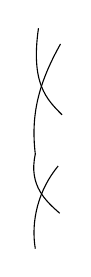
\begin{tikzpicture}[x=1cm,y=1cm]
\draw (0,2.8) .. controls (-.1,2.1) and (.1,1.9) .. (.3,1.7);
\draw (.28,2.6) .. controls (0,2.1) and (-.1,1.7) .. (-.04,1.2);
\draw (-.04,1.2) .. controls (-.13,.8) and (.1,.6) .. (.27,.45);
\draw (.25,1.05) .. controls (0,.75) and (-.1,.35) .. (-.04,0);
\end{tikzpicture}}}

\unsure{6|4}

\textcircled{1} $X$ \uline{régulier}, $\unsure{P|F}=\mathbb Q_{lX}$, $f$ immersion $(n=\dim\overline{f(X)})$.

On peut supposer $X\longrightarrow Y$ imm. \uline{ouverte}
\diagram{\begin{tikzcd}
&Y'\arrow[d,"h"]\\
X\arrow[ur,hook,no head,"g"]\arrow[r,hook,no head,"f"']&Y
\end{tikzcd}}
$Y'$ régulier, $Y'-g(X)=\deleted{\unsure{D}}h^{-1}(Y-X)=Z$ diviseur à croisements normaux $Z=\sum Z_i$.

\[
\deleted{\unsure{R}}R^*f_*(\mathbb Q_{lX})\Longleftarrow E^{pq}_2
=R^ph_*((R^qg_*(\mathbb Q_l)\unsure{(-1)|(-j)}))
\]
\[
R^qg_*(\mathbb Q_l)=\bigwedge^q\sum\mathbb Q_{lZ_i}
=\sum_{i_1<\cdots<i_q}\mathbb Q_{l\,Z_{i_1}\cap\cdots\cap Z_{i_q}}(-q)
\]
pur de poids $2q$

\margin{$X\subset$}

$E^{p0}_2=R^ph_*(\mathbb Q_{l\unsure{X'|Y'}})$ est eff$^{t}$ admissible de poids $\leq p=i$ niveaux $\leq\operatorname{Inf}(p,2n-2-\unsure{p}$

[\deleted{$\unsure{\leq2p}$} au complet si $p\geq n-1$]

\[
E^{pq}_2=\sum_{i_1<\cdots<i_q}R^pf_{Z_{i_1}\cap\cdots\cap Z_{i_q}*}(\mathbb Q_l)(-q)
\]
est eff. admissible de poids $\leq p+2q=i+q\deleted{\unsure{\leq}}\leq2n\deleted{\unsure{a}}$
de niveaux $\leq\operatorname{Inf}(p,2n-2q-p)$

\margin{$p\unsure{\leq}2(n\deleted{\unsure{a}}-q)\,/\,p$}
\margin{\textcircled{\unsure{V. l.|F. l.}} $i+q=$
$\boxed{\begin{gathered}p+2q\leq2n\deleted{\unsure{a}}\\q\leq n,2n-i\end{gathered}}$}

en tous cas, poids reste $\leq\deleted{\unsure{2}}\operatorname{Inf}(2i,2n-2$

niveaux \deleted{$\unsure{\leq i\rightarrow}$}
$\leq\operatorname{Inf}(i,2n-2-i)$

\margin{$p\leq n-1$\\$q\leq n$}

\[
\begin{array}{cc}p&\unsure{n+q|n-q}\\
\multicolumn{2}{c}{p+q\geq n}\end{array}
\]
\[
2(p-n+q)=2(i-n)\qquad 2n-2-
\]
\[
2(n-q)-p=\uline{2n-i}-q
\]

\figure{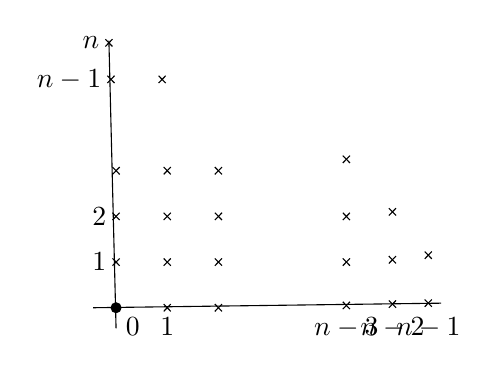
\begin{tikzpicture}[x=.65cm,y=.58cm]
\draw (-.45,0)--(6.35,.10);
\draw (0,-.45)--(-.14,5.85);
\fill (0,0) circle (2pt);
\foreach \x/\y in {0/1,0/2,0/3,-.10/5,-.14/5.8,1/0,1/1,1/2,1/3,.9/5,2/0,2/1,2/2,2/3,4.5/.05,4.5/1,4.5/2,4.5/3.25,5.4/.08,5.4/1.05,5.4/2.1,6.1/.10,6.1/1.15}
{\draw (\x-.07,\y-.08)--(\x+.07,\y+.08);
\draw (\x-.07,\y+.08)--(\x+.07,\y-.08);}
\node[below right] at (0,0) {$0$};
\node[below] at (1,0) {$1$};
\node[below] at (4.5,0) {$n-3$};
\node[below] at (5.4,0) {$n-2$};
\node[below] at (6.1,0) {$n-1$};
\node[left] at (0,1) {$1$};
\node[left] at (0,2) {$2$};
\node[left] at (-.1,5) {$n-1$};
\node[left] at (-.14,5.8) {$n$};
\end{tikzpicture}}

2.
